\documentclass{acm_proc_article-sp}
\usepackage{times}
\usepackage{microtype}
\usepackage{url}
\usepackage{graphics}
\usepackage{graphicx}
\usepackage{listings}
\usepackage{wrapfig}

\usepackage[utf8]{inputenc}
\lstset{basicstyle=\scriptsize \ttfamily, 
numbers=left, numberstyle=\tiny, stepnumber=1, numbersep=5pt}

\usepackage{caption}
\DeclareCaptionType{copyrightbox}
\usepackage{subcaption}

\usepackage{color}
\usepackage[pdftex]{hyperref}
\usepackage[]{algorithm2e}
\usepackage{todonotes}
%\usepackage[disable]{todonotes}%


\hypersetup{%
pdftitle={Towards an Open Question Answering Architecture},
pdfauthor={Marx Edgard and Usbeck Ricardo and  Ngomo Ngonga Axel-Cyrille and  H\"offner Konrad and Lehmann Jens and Auer S\"oren},
pdfkeywords={Question Answering},
bookmarksnumbered,
pdfstartview={FitH},
colorlinks,
citecolor=black,
filecolor=black,
linkcolor=black,
urlcolor=black,
breaklinks=true,
}
\newcommand{\comment}[1]{}
\definecolor{Orange}{rgb}{1,0.5,0}
\newtheorem{definition}{Definition}
\newcommand{\urlfn}[1]{\footnote{\scriptsize\url{#1}}}

\usepackage{enumitem}
\setitemize{noitemsep,topsep=-6pt,parsep=0pt,partopsep=0pt}

\pagenumbering{arabic}  % Arabic page numbers for submission.  Remove this line to eliminate page numbers for the camera ready copy
\usepackage{cleveref}


\widowpenalty = 10000
\clubpenalty = 10000
\begin{document}
%\crefname{section}{Section}{Sections}
%\crefname{figure}{Figure}{Figures}
%\crefname{table}{Table}{Tables}
% To make various LaTeX processors do the right thing with page size.
\special{papersize=8.5in,11in}
\setlength{\paperheight}{11in}
\setlength{\paperwidth}{8.5in}
\setlength{\pdfpageheight}{\paperheight}
\setlength{\pdfpagewidth}{\paperwidth}
\inputencoding{utf8}
% Use this command to override the default ACM copyright statement
% (e.g. for preprints). Remove for camera ready copy.
% \toappear{Submitted for review to WebSci 2012.}
% Ricardo Usbeck, Axel-Cyrille Ngonga Ngomo, Konrad H\"offner

\title{Towards an Open Question Answering Architecture}
%\title{Towards Open Interoperable Question Answering Modules} % Jens: just a title suggestion
\numberofauthors{3}
\author{
  \alignauthor Edgard Marx\\
    \affaddr{AKSW/BIS, Universit\"at Leipzig}\\
    \affaddr{PO Box 100920, 04109 Leipzig, Germany}\\
    \email{marx@informatik.uni-leipzig.de}
	\alignauthor Ricardo Usbeck\\
       \affaddr{Universit\"at Leipzig, IFI/AKSW}\\
       \affaddr{Unister GmbH, Leipzig}\\
       \email{usbeck@informatik.\\uni-leipzig.de}
	\alignauthor Axel-Cyrille Ngonga Ngomo\\
    \affaddr{AKSW/BIS, Universit\"at Leipzig}\\
    \affaddr{PO Box 100920, 04109 Leipzig, Germany}\\
    \email{ngomo@informatik.uni-leipzig.de}
	\and
	\alignauthor Konrad H\"offner\\
    \affaddr{AKSW/BIS, Universit\"at Leipzig}\\
    \affaddr{PO Box 100920, 04109 Leipzig, Germany}\\
    \email{hoffner@informatik.uni-leipzig.de}
  \and
	\alignauthor Jens Lehmann\\
    \affaddr{AKSW/BIS, Universit\"at Leipzig}\\
    \affaddr{PO Box 100920, 04109 Leipzig, Germany}\\
    \email{lehmann@informatik.uni-leipzig.de} \and 
  \alignauthor S\"oren Auer\\
    \affaddr{CS/EIS, Universit\"at Bonn}\\
    \affaddr{R\"omerstra\ss e 164, 53117 Bonn, Germany}\\
    \email{auer@cs.uni-bonn.de} 
}

\maketitle

\begin{abstract} 
Billions of facts pertaining to a multitude of domains are now available on the Web as RDF data.
However, accessing this data is still a difficult endeavour for non-expert users.
In order to meliorate the access to this data, approaches imposing minimal hurdles to their users are required.
Although many question answering systems over Linked Data have being proposed, retrieving the desired data is still significantly challenging.
% no significant results were being achieved in last years.
In addition, developing and evaluating question answering systems remains a very complex task.
To overcome these obstacles, we present a modular and extensible open-source question answering framework.
We demonstrate how the framework can be used by integrating two state-of-the-art question answering systems.
As a result our evaluation shows that overall better results can be achieved by the use of combination rather than individual stand-alone versions.
\end{abstract}

\section{Introduction}
\label{sec:introduction}

Since its inception, the Web has been used by millions of users with the aim of sharing, reproducing and linking information.
More and more structured data, e.g.,~using the Resource Description Framework (RDF), is made available by users, services and more recently sensors.
Consequently, machines are now empowered to use a large amount of data available on the Web.
Examples of such datasets are \emph{DBpedia}~\cite{dbpedia-swj}\footnote{\url{http://dbpedia.org}, version 3.9} and \emph{LinkedGeoData}~\cite{SLHA11}\footnote{\url{http://linkedgeodata.org}, version of March 23rd, 2014}, which encompass more than 1 billion triples each.
The main advantage of these datasets is that they represent a variety of knowledge across several domains.
For example, \textit{astronauts who took part in the Apollo 14 mission} can be easily retrieved from DBpedia.
Although this data is accessible, users still face difficulties when trying to retrieve the desired information using traditional methods.

In particular, state-of-the-art search engines fail to retrieve the set of resources intended by the user because most of them abide by the \textit{bag of words} paradigm.
% instead of the question answering (QA) approach to dealing with user needs.
%This is the case of RDF data search engines.
For instance, the query \textit{Apollo 14 astronauts} on search engines such as Sigma\footnote{\url{http://sig.ma}} and Sindice\footnote{\url{http://sindice.com}} will retrieve relevant documents rather than the desired set of resources.
Furthermore, in some engines fail finding a suitable answer, due to no full understanding of the input query or not properly indexed data in the underlying knowledge base.

Over the last years, several approaches for question answering (QA) based on the Web of Data have been proposed. 
However, retrieving the desired data is still significantly challenging.
Reported results from the Question Answering on Linked Data (QALD) benchmark\footnote{\url{http://greententacle.techfak.uni-bielefeld.de/~cunger/qald}} indicate that  only $\approx54\%$ of the given questions were correctly answered in QALD-1 and $32\%$ in the more difficult QALD-2 and QALD-3 benchmarks.

In this paper, we present \emph{openQA}, an open source question answering framework that combines several question answering systems.
The proposed framework can facilitate the evaluation by promoting the modularization and easy integration of new modules via a plug-in architecture. 
Moreover, our experiments reveal a considerable improvement of correct answers by combining question answering systems, i.e., $87.5\%$ using the QALD-3 benchmark.

The remainder of this paper is structured as follows.
\Cref{sec:rel} presents an background overview and related work.
\Cref{sec:design} introduces the framework architecture and its components.
\Cref{sec:impl} details the implemented components and used technologies.
\Cref{sec:eval} presents the achieved results.
Finally, \cref{sec:conc} concludes with an outlook on future work.
\\\\
\section{Background and Related Work}\label{sec:rel}

The World Wide Web Consortium recommend the use of Linked Data (LD) standard to represent and publish open data\footnote{\url{http://www.w3.org/standards/semanticweb}}.
The LD standard uses for the representation of data (facts, rules and their relationships) the \emph{RDF} format.
%This can formally be defined as follows:
%\vspace{-4.0mm}
%\begin{definition}[RDF definition]
%\label{def:triple}
%Let \emph{I}, \emph{B} and \emph{L} be an infinite disjoint sets of IRIs, Blank Nodes and RDF literals respectively.
%We set \textit{RDF terms} as being an infinite set of $m \in T$ where $T:=I \cup B \cup L$.
%Being the subject, predicate and object sets respectively defined by $S:={I \cup B}$, $P:={I}$ and $O:={I \cup B \cup L}$.
%A triple $t:=(m_s, m_p, m_o)$ is called an RDF \textit{triple} iff $m_s \in S$, $m_p \in P$, and $m_o \in O$.
%\end{definition}
%\begin{definition}[RDF Instance]
%\label{def:instance}
%A set of $n$ triples $E:=\{$ $t_0,$ $t_1,$ $t_2...t_n$ $\}$ is called RDF \textit{instance} $\Leftrightarrow \exists !$ $v_s \in S$ and $n \geq 1$.
%\end{definition}
%\begin{definition}[Knowledge base]
%\label{def:knowledgebase}
%The knowledge base $L$ is an union of a set of triples describing a set of classes $C$ and their instances $E$.
%$L \subset T : L:= C \cup E$
%\end{definition}
%\todo{Ricardo: classes and instances is not defined}

Question answering on linked data is an active and diverse research field with many existing research prototypes designed for different environments.
Systems running on a \emph{closed domain} are optimized for and only work on a specific knowledge base or field, like biology~\cite{biomedicalqa} or medicine~\cite{medicalqa}.
Since they do not need to integrate different schemas and knowledge bases and thus suffer less from ambiguity, they generally create faster and higher-quality results.
%Reuse and portability is however severely restricted.
However, closed-domain approaches lack flexibility.
Additionally, there are high costs when adapting such a system to a new domain or implementing a new system.
Thus, the research focus has been moved towards multi-purpose, open-domain QA systems like FREyA~\cite{freya} or hybrid approaches like TBSL~\cite{unger2012template} with a domain unspecific core and a domain specific, adaptable extension.

Question answering is a complex process which consists of many different steps, most of which have to be executed in a sequential manner and are thus called a pipeline.
Some of those steps, like natural language processing (NLP), which involves parsing and part-of-speech extraction can make use of mature, well performing tools.
No such simple solution exists however for the step of interpretation -- the process of extracting the meaning of a question.
%However, although the process of interpretation is very important on question answering systems, they do not rely on that.

%In the follows subsections we group the related work into two categories: (1) answer formulation and (2) presentation.
%Answer formulation (1) encompasses approaches for generating answers over natural language (NL) input queries whereas presentation, for better displaying the formulated answer.

%\subsection{Answer formulation}
FREyA~\cite{freya} is different from SPARQL driven systems and makes use of a combination of syntactic parse trees, phrases potentially representing ontologies as well as ontology concepts.
Phrases potentially representing ontology concepts, so-called \emph{Potential Ontology Concepts (POCs)} are identified by heuristics on the syntactic parse tree.
\emph{Ontology Concepts (OCs)}, are resources from an ontology that are identified matching their labels with phrases from the question without regarding its structure.
A consolidation algorithm then matches POCs to OCs.
In case of ambiguities, feedback from the user is asked.
Disambiguation candidates are created using string similarity in combination with WordNet synonym detection.
The system learns from the user selections, thereby improving the precision over time.
However, user feedback is rare and expensive.

Most frequently, QALD systems uses a set of predefined graph pattern templates in the interpretation process to generate SPARQL queries representing the input question.
The use of SPARQL queries enables the representation of a more complex semantic structure of the original natural language question,
going beyond the limitation of triple-only-based systems.
However, the strategy used to generate the graph patterns and consequently the SPARQL query differs significantly between approaches.
This is the case of \emph{SINA}~\cite{SHE+13}, \emph{TBSL}~\cite{unger2012template} and \emph{Casia}~\cite{clef2013casia}.

\emph{SINA} is a question answering system that uses the knowledge base itself to formulate the graph pattern templates.
The system deals with the input query as being a set of keywords, which enable the interpretation of keyword as well as full question fashion queries.
In order to prune the number of generated graph pattern templates, \emph{SINA} uses a statistical Hidden Markov model.

\emph{TBSL} is another template-based question answering system for LD.
Different from other approaches, \emph{TBSL} uses an entity identification and predicate detection method to fill the slots of the previosuly defined SPARQL template query with data extracted from the original query.

\emph{Casia}~\cite{clef2013casia} generates the graph pattern templates by using the question type, named entities and POS tags techniques.
The generated graph patterns are then mapped to resources using Wordnet, PATTY and similarity measures.
Finally, the possible graph pattern combinations are used to build SPARQL queries.

As each of these systems has its strengths and weaknesses, we move a step further, adopting a composed solution.

\section{Framework Design}
\label{sec:design}

\begin{figure*}[bht]
	\centering
	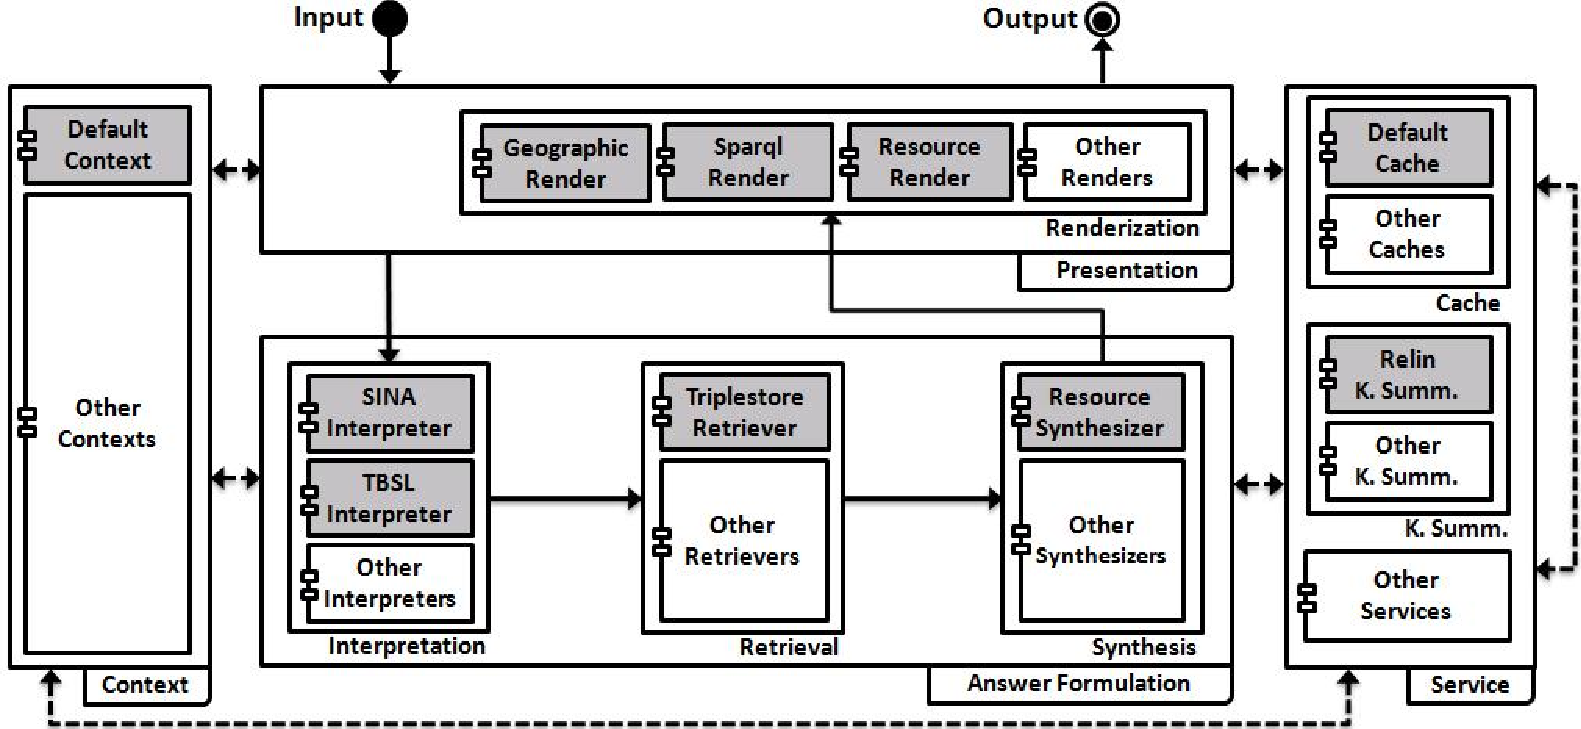
\includegraphics[width=.97\textwidth]{images/architecture.pdf}
	\caption{openQA Architecture Overview.}
	\label{fig:architecture}
	\vspace{-4.0mm}
\end{figure*}
We propose a framework for combining different approaches to question answering.
The design was made taking into account the architecture of classic and over linked data QA systems, search engines, smart assistants as well as hybrid systems such as IBM Watson \footnote{\url{http://www.ibm.com/smarterplanet/us/en/ibmwatson}}.
In the following, we explain our \emph{openQA} framework architecture which consists of four main modules comprising several sub modules, see~\Cref{fig:architecture}.
The framework has a main work-flow comprising four stages (\emph{interpretation}, \emph{retrieval}, \emph{synthesis},  %and %\emph{resolution}, 
\emph{renderization}) and adjacent modules (\emph{context} and \emph{service}).
The adjacent modules are intended to be accessed by any of the components of the main work-flow.

One of the biggest challenges in realizing a generic framework is how to combine different approaches.
To tackle this challenge, the framework was designed in a plug-in architecture style.
Plug-in architectures are known for promoting modularization and easy integration.
We aim that the openQA architecture allows to support the diversity of many existing Linked Data question answering systems. % and is organized as follows.
\emph{openQA} is organized as follows:
\vspace{-4.0mm}
\paragraph{\textbf{Answer Formulation}} The core module comprises the \emph{answer formulation} process, its purpose is to receive an input query and deliver the most probable answer candidates.
The answer formulation process is composed by four different stages:
\vspace{-3.0mm}
\begin{enumerate}
	\item \emph{Interpretation} The first and crucial step of the core module is the \emph{interpretation}. 
	Here, the framework attempts to generate a formal representation of the (intention behind the) input question.
	By these means, it also determines how the input question will be processed by the rest of the system.	
	Because the interpretation process is not trivial, there is a wide variety of techniques that can be applied at this stage, such as tokenization, disambiguation, internationalization, logical forms, semantic role labels, question reformulation, coreference resolution, relation extraction and named entity recognition amongst others.
	Most of these technologies are well understood and will not be discussed here.
	The interpretation stage can generate one or more interpretations of the same input in different formats such as SPARQL, SQL or string tokens.
	\item \emph{Retrieval} After an interpretation of the given question is generated, the \emph{retrieval} stage extracts answers from sources according to the delivered interpretation format or content.
	For instance, one of the outputs of the interpretation can be: 
	(1) a SPARQL query which can be handled by a triple store;
	(2) an SQL query which will be processed by a relational database, or;
	(3) a set of keywords that can be sent to a document-based search engine.
	Specific interpretations can also be used for extracting answers from sources such as web services.		
	\item \emph{Synthesis} %After a set of answer candidates be founded by the retrieval stage, a synthesize stage is required.
	Answers may be extracted from different sources, be ambiguous and redundant.
	To alleviate this issues the \emph{Synthesis} stage processes all information from different retrieval sub-modules.
	Results that appear multiple times are fused with an occurrence attribute that helps to rank, cluster and estimate the confidence of the retrieved answer candidates.
	The \emph{Synthesis} process is closed by \textit{\Cref{def:synthesis}}.

\end{enumerate}
\vspace{-5mm}
\begin{definition}[Synthesis]
\vspace{-2.0mm}
\label{def:synthesis}
Let $R_1, \ldots, R_n$ be the result sets generated by different search. 
The result of the synthesis process is a duplicate-free result set $R=\bigcup\limits_{i=1 \ldots n} R_i$. % such that $\forall x \in R$ and $y \in R$ we will have $x = y$. 
The ranking of the results in $R$ is left open to the user but must be specified by the means of an injective function $pos$ which maps each $r \in R$ to exactly one value between 1 and $|R|$.
 
%Considering a series of answer candidates $R$ of type $w$, $R:=\{w_0,w_1,w_0,$ $w_2...w_n\}$, composed by a series of \textit{RDF Terms} of type $t \in T$ retrieved from one or more SPARQL queries.
%The synthesis process is covered by the function $synthesis(R)=R'$, where the position of $w' \in R'$ is given by the function $pos(w')$ and the following holds:
%\[\forall w \in R, \exists! w' \in R', w=w'\]
\vspace{-5.0mm}
\end{definition}

%The retrieved answer candidates can be from different explored graphs and formats: video, image, document and resource.	
%The syntheses stage is also designed for cluster all the related entity information.
%	\item \emph{Resolution} The last stage is the resolution.
%	The resolution stage can apply filters to remove noise, choose or re-arrange the most promising candidates.
%	The usage of machine learning is also encouraged.
%	Machine learning allows the system to better rank and select the synthesized candidates which allows the system to produce better results in future queries.
\vspace{-3.0mm}
\paragraph{\textbf{Renderization}}
Typically a knowledge base comprises data in several types and formats.
Each type of information demands a specific display style to deliver the best possible amount of information to the user.
In the proposed architecture the concepts of answer \emph{formulation} and \emph{presentation} are detached.
The \emph{renderization} module encapsulates the answer presentation and comprises one or more renders that work as widgets.
That is, each widget plugged to the \emph{renderization} module can be used to render one type or format of data.
\vspace{-4mm}

\paragraph{\textbf{Context}} Users context can help the answer personalization providing information such as who or where is the user, what is the preferred language or if the question is one of a series of related previous questions.
To enable the system to produce better answers the \emph{context} module can store users information, such as location, statistics and previous queries.
\vspace{-4mm}
\paragraph{\textbf{Services}} The \emph{services} modules are designed to be easily accessed by the components. 
They intend to facilitate the encapsulation, addition and sharing of application functionalities between the modules i.e.:% so it can be shared amongst them.
\vspace{-3.0mm}
\begin{enumerate}
	\item \emph{Cache} The result of a determined parameter in a function can be required multiple times. The \emph{cache} service intends to provide efficiency while prevents the execution of the same process multiple times.
	It stores the results of processes in order that future requests to the same process can be executed faster.
	\vspace{-2.0mm}
	\item \emph{Knowledge Summarization}
	Currently, the \emph{DBpedia}\footnote{\url{http://wiki.dbpedia.org/About}} dataset comprises millions of facts distributed over millions of entities, but not all this data is useful for users.
	\emph{Knowledge Summarization} has an important role in knowledge presentation.
	Knowledge summarization refers to a combination of two techniques, set and entity summarization.
	Set and entity summarization consist of the use of heuristics to rank respectively entities and their attributes.
	\vspace{-4.0mm}
\end{enumerate}

\begin{figure}
	\centering
	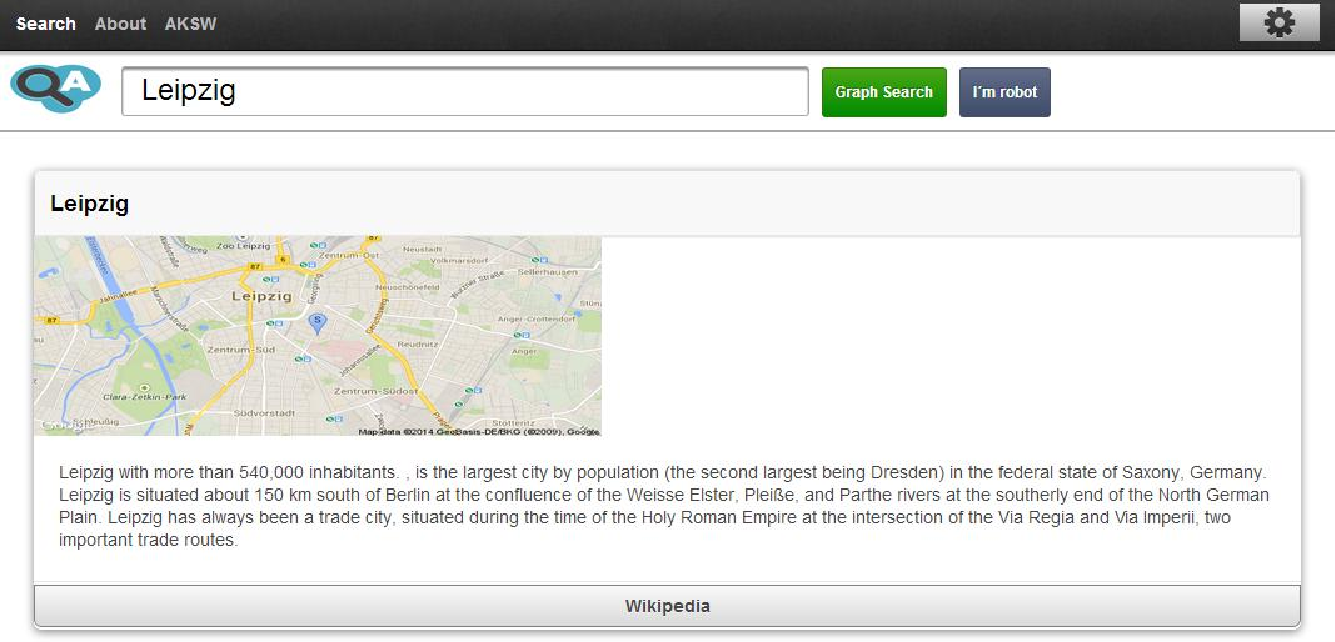
\includegraphics[width=\columnwidth]{images/sample_page.pdf}	
	\caption{Screenshot of the demo available at \url{http://openqa.aksw.org}.}
	\label{fig:demo}
	\vspace{-4.0mm}
\end{figure}

\section{Implementation}
\label{sec:impl}

The framework is implemented as open-source and additionally provides several built-in components and information about: (1) possible log messages, (2) used memory, (3) errors as well as (4) answered and not answered queries.
\Cref{fig:architecture} gives an overview of the implemented modules in gray.
Moreover, a test integration framework was developed in order to run evaluation queries on \emph{openQA} and the underlying modules.

\paragraph{\textbf{Combining Approaches}}
\vspace{-4.0mm}
%The remaining of the framework is structured as follows.
Regarding \emph{Knowledge Summarization}, an algorithm based on \emph{Relin}~\cite{cheng2011relin} has been added.
\emph{SINA} and \emph{TBSL} were combined as interpretation modules.
The framework can handle SPARQL queries over a retrieval component based on the \emph{Jena}\footnote{\url{http://jena.apache.org}} client.
The synthesis module is inspired by~\cite{conf/aswc/LopezNFSUM09} and formalized by \Cref{def:synthesis} in which $pos(r) = - \log(|r|/|R|)$, i.e., the more occurrences an answer has, the more confidence it provides.
The renderization module of \emph{openQA} uses \emph{Infograph}.
\emph{Infograph} is a render API developed for \emph{openQA} that can render (1) SPARQL queries, (2) literals and (3) entities from knowledge bases.
Infograph is capable of differentiating entities with and without geographic information as well as automatically generate entity descriptions based on their attributes via \emph{SPARQL2NL}~\cite{sparql2nl-demo}, in case the entity does not have a description.

\section{Evaluation}
\label{sec:eval}

The evaluation of the described framework was performed measuring improvement of correct answered queries in QALD-3 by combining the participant systems.
Furthermore, the framework was assessed with the fourth version of the same benchmark (QALD-4), by using stand-alone versions of \emph{TBSL} and \emph{SINA} as well as a combination of both.
All evaluations were executed over the multilingual tasks.
The correctness and incorrectness synthesized answer from different systems is given by logical conjunction.
According to QALD benchmark the result from the synthesis operations should be equal to the given correct answer set $C$ otherwise is considered incorrect.
\[\forall x \ C(x) \iff \bigvee_{i=1}^n R_i(x)\]

\vspace{-4.0mm}
The QALD-3 evaluation (\Cref{fig:combining}) shows that a significant improvement of correct answers can be achieved (87.5\%) by using a theoretical combination of all the participant systems.

Regarding QALD-4, we measure a combination of the current implemented versions of \emph{SINA} and \emph{TBSL} (trained respectively using QALD-2 and QALD-1). 
As both systems were still under major revision, the tests were focused in how much improvement could be achieved under their combination. 
The results reveal that a combination of both systems is also better than a stand-alone versions, leading to an improvement of 11\% in correct answered queries.

\begin{figure}[h]
	\centering
	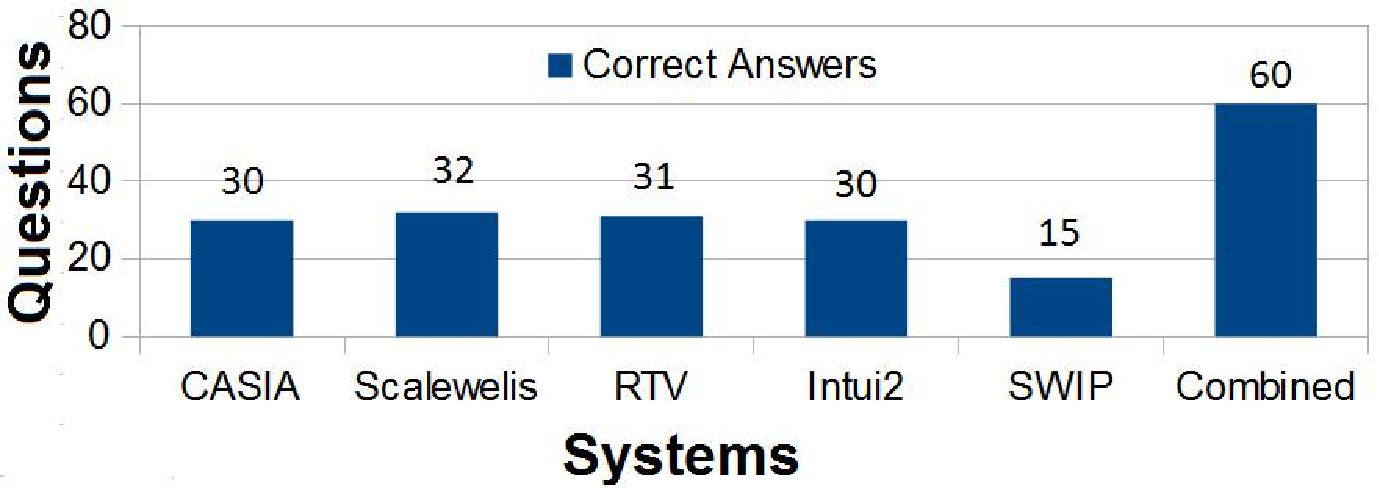
\includegraphics[width=\columnwidth]{images/right_answers.pdf}	
	\caption{Correct answers on combining QALD-3 systems.}
	\label{fig:combining}
\end{figure}

The framework (\Cref{fig:demo}) is available over two public instances,
one using \emph{SINA} (\url{http://sina.aksw.org}) and another using both, \emph{SINA} and \emph{TBSL} (\url{http://openqa.aksw.org}).
As the live instances rely on the public \emph{DBpedia} endpoint, the user's experience can be affected by instabilities.
Regarding this, a demo video is also available at \url{http://www.aksw.org/Projects/openQA}.

\vspace{8.0mm}
\section{Conclusions and Future Work}
\label{sec:conc}

The proposed architecture is part of a larger research agenda which aims to define and develop a common framework for question answering systems.
%It is also a complement of work of set of specialists and technologies.
Therefore, we have implemented several components, which are open source and can be downloaded, plugged and extended \footnote{\url{http://aksw.org/Projects/openQA}}.
The achieved results indicate that the \emph{openQA} architecture can be used as a base for developing, combining and evaluating question answering systems.
The next efforts will consist of integrating unstructured sources, such as text extracted data from web pages and document bases.
Furthermore, we want to extend the implemented modules with non-commercial APIs from other question answering systems and evaluate them against several well-know benchmarks. 

\textbf{Acknowledgments}
\begin{wrapfigure}[2]{r}{4.4cm}
 \vspace{-8mm}
 {
\includegraphics[height=1cm]{esf.pdf}}\,{
\includegraphics[height=1cm]{7fp.png}}
\end{wrapfigure}
This work has been supported by the ESF and the Free State of Saxony and the FP7 project GeoKnow (GA No. 318159) and by CNPq, under the program Ciências Sem Fronteiras.
\vspace{-5mm}
\bibliographystyle{abbrv}
\bibliography{aksw,references}
\end{document}
